
%(BEGIN_QUESTION)
% Copyright 2011, Tony R. Kuphaldt, released under the Creative Commons Attribution License (v 1.0)
% This means you may do almost anything with this work of mine, so long as you give me proper credit

Geothermal power plants rely on multiple ``production wells'' drilled deep into the earth to extract hot fluids which are then used to drive steam turbines.  The following control system cascades the pressure controller's output to three flow control loops in order to ``balance'' the production rates of three different wells rather than over-use or under-use any one of them:

$$\includegraphics[width=15.5cm]{i03495x01.eps}$$

The ratio value for each production well is determined by operations engineers, their sum totaling to 100\%.

\vskip 10pt

Suppose an engineer makes a mistake one day, setting the ratio for well \#1 at 25\%, the ratio for well \#2 at 41\%, and the ratio for well \#3 at 43\%.  Obviously, these three ratio values do {\it not} add up to 100\%.  Calculate the actual flow ratios of wells \#1, \#2, and \#3 as percentages of the total (true) flow entering the HP separator vessel.

\vfil 

\underbar{file i03495}
\eject
%(END_QUESTION)





%(BEGIN_ANSWER)

This is a graded question -- no answers or hints given!

%(END_ANSWER)





%(BEGIN_NOTES)

Obviously, these three percentages add to make a value greater than 100\% (25\% + 41\% + 43\% = 109\%).  However, we may still calculate the true percentage of flow as a fraction of this greater total:

\vskip 10pt

Well \#1 true flow ratio = $25 \over 109$ = 22.94\%

\vskip 10pt

Well \#2 true flow ratio = $41 \over 109$ = 37.61\%

\vskip 10pt

Well \#3 true flow ratio = $43 \over 109$ = 39.45\%

\vskip 10pt

The necessity of calculating the true percentages this way becomes clearer to see if we apply the problem-solving technique of {\it simplifying the problem}.  Imagine that the engineer set all three ratio settings at 100\%.  Thus, each production well valve would operate to give full-scale flow (according to the flow transmitters).  However, 100\% + 100\% + 100\% = 300\%, so we cannot take the individual 100\% settings at face value.  The fact that all three wells are operating at ``100\%'' flow means that each one actually contributes one-third ($100 \over 300$) of the total flow.  Therefore, we may conclude from this simplification that the proper way to perform the true percentage calculation is to calculate the ratio of each setting as given compared to the sum total of all the settings.

%INDEX% Process: geothermal power plant

%(END_NOTES)


